\documentclass[11pt]{report}

% sensible specification of margins, etc.
\usepackage[paperwidth=8.5in,paperheight=11in]{geometry}
\geometry{inner=1.0in, outer=1.5in, top=1.0in, bottom=0.5in,
  includefoot}
\geometry{twoside}

% for displaying graphics
\usepackage[]{graphicx}
% where can I find the graphics that will be imported for this version
\graphicspath{{./figures/}}

% running headers
\usepackage{fancyhdr}
\fancyhead{}
\fancyfoot{}
%\fancyhead[CO,CE]{---Draft---}
\fancyhead[LO,RE]{\it The G2Cam Toolkit}
\fancyhead[LE,RO]{\slshape \rightmark}
\fancyfoot[C]{\thepage}
%\fancyfoot[LE,RO] {\slshape \rightmark}
%\fancyfoot[LO,RE] {\slshape \leftmark}

% use modern and attractive fonts
\usepackage{fontspec}
\setmainfont[Mapping=tex-text]{Times New Roman}
\setsansfont[Mapping=tex-text]{Arial}
%\setmonofont[Scale=0.85]{Courier New}
\setmonofont[]{Courier New}
%% \setmainfont[Mapping=tex-text]{Bitstream Vera Serif}
%% \setsansfont[Mapping=tex-text]{Bitstream Vera Sans}
%% \setmonofont[Scale=0.85]{Bitstream Vera Sans Mono}

% Save space in headings
%% \usepackage[small,compact]{titlesec}
%% \titlespacing{\section}{0pt}{*0}{*0}
%% \titlespacing{\subsection}{0pt}{*0}{*0}
%% \titlespacing{\subsubsection}{0pt}{*0}{*0}

% provides itemize* environment
\usepackage{mdwlist}
% for tables with paragraphs
\usepackage{tabularx}

% for URLs without links
\usepackage{url}
  
% for code listings
\usepackage{listings}
\usepackage{color}
\usepackage{textcomp}
\lstset{
	%backgroundcolor=\color{lbcolor},
	tabsize=4,
	%rulecolor=,
	language=Python,
        basicstyle=\scriptsize,
        upquote=true,
        aboveskip={1.5\baselineskip},
        columns=fixed,
        extendedchars=true,
        breaklines=true,
        prebreak = \raisebox{0ex}[0ex][0ex]{\ensuremath{\hookleftarrow}},
        %frame=single,
        showtabs=false,
        showspaces=false,
        showstringspaces=false,
        identifierstyle=\ttfamily,
        keywordstyle=\color[rgb]{0,0,1},
        commentstyle=\color[rgb]{0.9,0.0,0.133},
        stringstyle=\color[rgb]{0.127,0.5126,0.941},
}
\usepackage{verbatim}
\newenvironment{myverbatim}
  {\setlength{\parskip}{0pt}\verbatim}
  {\endverbatim}

%\raggedright

\setlength{\parindent}{0cm}
\setlength{\parskip}{1em plus0.5em minus0.5em}

\setlength{\marginparsep}{0.35in}
\setlength{\marginparwidth}{1.5in}

\title{The G2CAM Subaru Instrument Interface Framework} 
\author{Eric Jeschke\\
{\tt eric@naoj.org}\\
\\
Observation Control Software Group\\
Subaru Telescope\\
National Astronomical Observatory of Japan}

\pagestyle{fancy}    

\begin{document} 

\maketitle 

\begin{abstract}
This document addresses an audience of software developers interested in
writing software for interfacing an observation instrument to Subaru
Telescope's Observation Control System (OCS). Some basic understanding
of software development principles as well as a general familiarity with
observatory infrastructures is assumed. 
\end{abstract}

\tableofcontents
\setcounter{tocdepth}{3}

\newpage

%%%%%%%%%%%%%%%%%%%%%%%%%%%%%%%%%%%%%%%%%%%%%%%%%%%%%%%%%%%%% 
\chapter{Introduction}
\label{sh:intro}

% fig: showing the default configuration
\begin{figure}
  \begin{center}
    \begin{tabular}{c}
      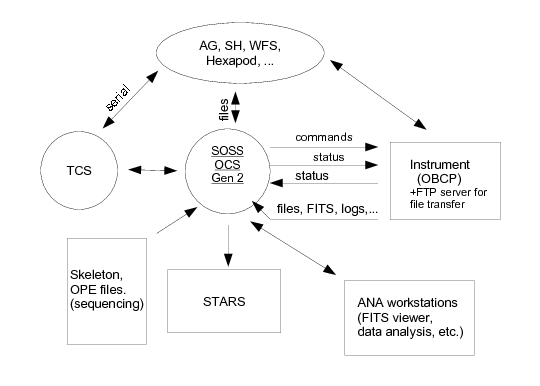
\includegraphics[width=5in]{OCS_schematic.png}
    \end{tabular}
  \end{center}
  \caption[example] 
%% %>>>> use \label inside caption to get Fig. number with \ref{}
          { \label{fig:obssubsys} 
            Subaru Telescope Subsystem Overview
             (figure courtesy Scot Kleinman). } 
\end{figure} 

Subaru Telescope's distributed control system is based on four
fundamental subsystems, illustrated by Figure \ref{fig:obssubsys}: 
\begin{itemize}
\item There is the Telescope Control System which controls the basic
movements of the telescope and its mechanical components, as well as
those of the dome, etc. 

\item There is the Instrument Control System, which encompasses all of
the computer control components of an instrument. 

\item There is the data archive system, known as STARS (Subaru Telescope
ARchive System). 

\item At the center of these systems is the Observation Control System,
which interfaces to the three systems referred to above, as well as
providing the human interfaces to the operators and observers. Subaru's
OCS is known as ``Gen2'' (so called because it is the second generation
OCS for Subaru).  
\end{itemize}

At Subaru, the interface between the instrument control system and the
observation control system is handled by a top-level computer referred
to as the OBCP (OBservation Control Processor). The OBCP is typically a
Unix/Linux-based system that is the locus for commands, status, and data
files transferred between the two systems. 

On the right-hand side of Figure \ref{fig:obssubsys}, you can see the
OBCP and its interfaces with the OCS. This interface encompasses four
basic ``channels'': 
\begin{itemize}
\item Commands to the instrument from the OCS and the instrument's responses;

\item Requests for external status data from the instrument to the OCS
and the OCS's replies with that requested status. 

\item Transfers of internal status data of interest from the instrument
to the OCS for distribution to other subsystems, and 

\item Requests for transfers of data files created by the instrument to
the OCS, and the OCS's replies about the results of transferring the
files. All files transferred from the instrument are automatically
archived from the OCS via STARS. 
\end{itemize}

\chapter{G2CAM}
G2CAM is a object-oriented software framework, written in Python, for
interfacing top-level instrument control systems to Subaru Telescope's
Observation Control System. As shown in the diagram in Figure
\ref{fig:obssubsys}, G2CAM implements and abstracts the low level
interfaces used for commands to, status transfer to and from, and file
transfer from, the instrument's top level computer, or ``OBCP''. Using
this framework, developers can write multi-threaded applications to
interface with the OCS with a quite high level of abstraction. The
top-level G2CAM module can be written to interface with instrument's
own internal subsystems in a variety of ways, including Python classes
and functions, embedded C code, FIFOs, sockets, files, shared memory,
etc.

\section{Obtaining and Installing G2CAM}

\subsection{Requirements}
G2CAM will run happily with either python 2.7 or 3.4+.  It doesn't have
any external requirements other than the Python standard library.
For some testing purposes, it may be helpful to have {\tt astropy}
installed.  

\subsection{Getting G2CAM}
g2cam is publicly available in a {\tt git} repository from the
\url{GitHub.com} web site.  To fetch it:
\begin{verbatim}
  $ git clone http://github.com/naojsoft/g2cam
\end{verbatim}

\subsection{Installation}
Install like any other python package:
\begin{verbatim}
  $ cd g2cam
  $ python setup.py install
\end{verbatim}
Be sure to use the version of python that you want to run g2cam with
when you do the install (e.g. if you have both python 2 and python 3
installed).

If you want to install it to a custom directory, please see the
{\tt README} file at the top level of the source tree, which describes
installation for more complicated setups.

For running instructions, please see Chapter \ref{ch:running} or the
above mentioned {\tt README} for the most current instructions.  

\section{The G2CAM API}
To interface with the G2CAM framework, a Python module is created which
defines at least one class inheriting from the BASECAM class, which is
defined in the SIMCAM package\footnote{G2CAM's predecessor was known as
SIMCAM; that is why the top-level package is named as such.}.
This inheritance provides the class with some abstract superclass
methods and attributes that will normally be overridden by the subclass. 

\begin{verbatim}
#
# My new instrument
#
from SIMCAM import BASECAM, CamError, CamCommandError
...

class MYCAM(BASECAM):

    ....

\end{verbatim}
There are several example modules included for real instruments that are
used at Subaru. Examining these example modules you will see what
arguments are necessary for the class constructor (also described in the
section below ``Putting it all together: the G2CAM cam'').
For methods defined inside the class there are a number of useful
convenience methods for logging, running concurrent tasks and
interacting with the OCS. 

\section{Command processing}
Command processing in the G2CAM framework is based on an event-driven
callback model that will be familiar to most developers. By simply
defining non-private methods in the class, those functions immediately
become available commands to the OCS. For example 
\begin{verbatim}
class MYCAM(BASECAM):
    ...
    ...
    #######################################
    # INSTRUMENT COMMANDS
    #######################################

    def snap(self, frameid=None, itime=10.0):

        self.logger.debug("snap called.")
        ...
        ...

\end{verbatim}
Defines a new instrument MYCAM that contains an callable command called
snap (presumably some kind of exposure command), with parameters frameid
and itime. From the OCS side, commands are case-insensitive, so the
command might be invoked as snap, SNAP, Snap, sNAp, etc. 
On the G2CAM side the method name should be defined in lower case. 

Parameters should be defined as Python keyword arguments, with default
values that will be assigned if they are not supplied at the time of
invocation. 

The command does whatever it needs to do (calling other methods,
etc). There are several possible scenarios for command completion: 
\begin{itemize}
\item The method raises a generic exception. In this case it will be
caught and reported as a command completion with error to the OCS (using
the exception error string). A traceback is also logged. 

\item The method raises a CamCommandError exception (or a subclass
thereof). This is the preferred way of signaling an error. An error is
reported to the OCS using the exception string and no traceback is
logged. 

\item The method returns normally and the result is an int or a tuple of
(int, str). In this case, the integer is interpreted as a return code: 0
is success, and non-zero is an error. In the tuple form, the string
provides a diagnostic of success or failure message. 

\item The method returns normally, but the result is not an int or a
tuple of (int, str). In this case, the command is assumed to have
completed successfully, and a success code and generic diagnostic is
returned to the OCS. If a Python method exits a method by ``falling off
the end'' (i.e. no return statement), the return code is None.
That covers this particular case. 
\end{itemize}
Note that since the framework is multi-threaded, executing a command
does not prevent other commands from being received and processed.
Although the API methods of the G2CAM framework are thread-safe, it is
up to the developer to make sure that shared instance 
state in the subclass is protected via standard thread-safety techniques
such as semaphores, locks, condition variables, etc. 
The threading and Queue packages in the standard Python library provides
many useful classes for this purpose. 

Although commands are typically driven from the OCS side, an instrument
can set up it's own autonomous command invocations. 
The G2CAM framework includes a thread pool and some common methods for
executing a method or function on it (see section below ``Creating
concurrent tasks'').
Alternatively you may choose to create and invoke threads using
the Python threading library directly. Either way, a method can be
spawned off into an independent self-timed loop for handling periodic
tasks. 

Since Python is a dynamic, interpreted language, the turnaround time for
developing and debugging new commands is very fast. Simply add new
methods to the module in an editor and restart g2cam. 

\section{Requesting external status}
Although commands are typically initiated from the OCS side, requests
for status values are initiated from the instrument side. A typical
example is when taking an exposure, the instrument needs the telescope
pointing values for RA and DEC before and after the exposure for the
purpose of creating a FITS file. 

The G2CAM framework provides a method in a delegate object for fetching
external status values. Let's enhance our snap method to illustrates how
it is used: 
\begin{verbatim}

    def snap(self, frameid=None, itime=10.0):
        """
        A command to open the shutter of the camera and begin exposure.
        """
        ...
        
        # Create a dictionary, whose keys are status aliases we want
	statusDict = {'STATS.RA': None, 'STATS.DEC': None}

        try:
            self.ocs.requestOCSstatus(statusDict)

        except CamError, e:
            # Some kind of error occurred--bail out
            raise CamCommandError("Failed to obtain status: %s" % str(e))

        # Successful call, get values
        ra, dec = (statusDict['STATS.RA'], statusDict['STATS.DEC'])
        self.logger.debug("ra=%s, dec=%s" % (ra, dec))

        # Do other snap stuff...
        ...
        ...

\end{verbatim}
There are a couple of things to note about this example. One is the use
of the logging facility. If the run-time logging level is set to include
debug, then the information about the ra and dec will be logged. The
second is the use of Exceptions to catch and signal errors. Note that
the call to requestOCSstatus() is wrapped in a try/except clause, and
that we re-raise the error as a CamCommandError if we run into
trouble. We could also simply return an error code, or an error code and
message, as described in the section on command processing. Thirdly,
note how we create a dictionary with the keys of the OCS status items
for which we want values. These keys are called status aliases. There
are hundreds upon hundreds of them. Someday hopefully we will have a
manual to describe them all. Until then, your best bet is to examine the
code in the example cam modules or ask a member of the Subaru OCS
software team or a Subaru support scientist what the aliases are for the
status values you need, and what the type of those values are. 

The call to self.ocs.requestOCSstatus() fills in the dictionary with the
values fetched from the OCS. The values are given the appropriate type
for the kind of status that they are (float, int, string, etc.). In this
case, the STATS.RA and STATS.DEC values are defined as string values in
the OCS, which is why they are returned as such. Of course, convenience
methods could be defined for fetching different sets of commonly needed
status items and massaging them as appropriate. 

We should point out that in many cases, an attempt to fetch a valid
status alias that has no currently defined value (or even an invalid
status alias) may not raise an exception. Instead, that particular
dictionary element will have an error value in it, and the whole status
call will succeed, because the OCS system returns these error values
without signaling an overall error to the low level interface. These
individual errors may be checked for by comparing the values with the
following method (compare to above): 
\begin{verbatim}

    def snap(self, frameid=None, itime=10.0):
        """
        ...
        ...

        try:
            self.ocs.requestOCSstatus(statusDict)

        except CamError, e:
            # Some kind of error occurred--bail out
            raise CamCommandError("Failed to obtain status: %s" % str(e))

        results = self.ocs.validateStatus(statusDict)
        if len(results) > 0:
            self.logger.error("Values are invalid for: %s" % str(results))
            for alias in results:
            ...
            ...
        ...
        ...

\end{verbatim}
The code could then examine the particular aliases to see if it is
possible to proceed without them. 

\section{Distributing instrument status}
Instruments may want to distribute internal status that may be of
interest to external parties. In particular, if the skeleton files or
observation plan files need to conditionally do something based on the
state of the instrument, this is usually handled by examining the most
recent status that was sent by the instrument. Like status requests,
status distribution is initiated by the instrument side, and not the
OCS. Status may be distributed at any time by the instrument, and the
OCS system will absorb it, process it and make it available through the
OCS status system. 

\subsection{Setting up instrument status tables}
Status distribution is a little more complicated than status requests
due to the way that status is currently handled in the OCS system (by
tables that are essentially packed buffers). This underlying buffer
interface was unfortunately exposed to the API in the first generation
OCS, which required instruments to pack their own status buffers, and
exposed the concept of separate status tables. This internal
representation may change in Gen2. Currently, the interface requires a
little bit of boilerplate code to set up the linkage between the G2CAM
status values and what is expected on the OCS side. 
\begin{verbatim}

    #######################################
    # INITIALIZATION
    #######################################

    def initialize(self, ocsint):
        super(G2CAM, self).initialize(ocsint)

        self.logger.info("initialize() called")

        # Grab my handle to the OCS interface.
        self.ocs = ocsint

        # Get instrument configuration info
        self.obcpnum = self.ocs.get_obcpnum()
        self.insconfig = self.ocs.get_INSconfig()

        ...
        ...

        # Get our 3 letter instrument code and full instrument name
        self.inscode = self.insconfig.getCodeByNumber(self.obcpnum)
        self.insname = self.insconfig.getNameByNumber(self.obcpnum)
        
        self.statusTblName = ('%3.3sS0001' % self.inscode)

        # Prepare the internal to Gen2 status mapping
        d = { 'status': '%s.STATUS',
              'mode':   '%s.MODE',
              'count':  '%s.COUNT',
              'last_frame': '%s.LFRAME',
            }
        mapping = {}
        for key, alias in d.items():
             mapping[key] = alias % self.inscode

        # Register my status items.
        self.mystatus = self.ocs.addStatusTable(self.statusTblName,
                                                ['status', 'mode', 'count',
                                                 'last_frame'],
                                                 mapping=mapping)
        
        ...
        ...

\end{verbatim}
This code example shows the initialize method, which is part of the
standard boilerplate code used in initializing the instrument module
(see Putting it all together: the G2CAM cam). When called, the
parameter ocsint is a handle to the OCS interface delegate object. After
calling the superclass constructor, the method stores this away in its
internal state in the variable ocs (you encountered this variable in
earlier examples, now you see where it came from). 

Using that handle, the initialize method can now invoke delegate calls
to the interface to accomplish various things. First, it finds out it's
own OBCP number (all Subaru instruments are enumerated), followed by
it's code (official 3-letter acronym) and full name (canonical name). 

It then constructs a table name (which must exist on the OCS side; the
example shows the canonical table name for an instrument), a table
format (a format string describing how to pack the status values into
the buffer) and then makes a call to addStatusTable() to create a table,
containing the listed status elements, and connecting it to the format
string. 

\subsection{Getting and setting internal status}
Beyond the boilerplate code, status values can be set any time, anywhere
in the module by simply assigning the values to the status table object
(you can also create multiple table objects) in dictionary style, or
using any of several convenience methods: 
\begin{verbatim}

        ...
        # dictionary style interface...
        self.mystatus['status'] = 'ALIVE'
        self.mystatus['last_frame'] = ''

        # Convenience method, with keyword arguments:
        self.mystatus.setvals(status='ALIVE', last_frame='')
        ...
        # Convenience method, with dictionary:
        statusDict = {'status': 'ALIVE', 'last_frame': ''}
        self.mystatus.store(statusDict)
        ...

\end{verbatim}
The advantage of using the convenience functions is that it ensures that
all the listed status items are updated together, and not intermixed if
another thread is also updating, or reading, status. 

Similarly, to read your own (instrument) status, you can either access
the items dictionary style, or use convenience methods: 
\begin{verbatim}

        ...
        # dictionary style interface...
        last_frame = self.mystatus['last_frame']

        # Multiple items can be fetched, atomically as a group
        (status, last_frame) = self.mystatus.fetchList(['status',
                                                        'last_frame'])

        # Or you can use a dict, to get them as a group
        statusDict = {'status': None, 'last_frame': None}
        self.mystatus.fetch(statusDict)
        ...

\end{verbatim}
Again, using the convenience methods insures that all the status items
are fetched as a group, atomically. The goal here is to abstract as much
as possible the OCS internal representation of status. For Gen2, it is
likely that the old status interface will be retained for some
time. However, using this abstraction means that only the boilerplate
code in initialize will likely need to be changed for an all new Gen2
status interface. 

\subsection{Transmitting internal status}
Status is not transmitted (distributed) until an explicit call is made
to do so. You might define a method to export the status like so: 
\begin{verbatim}

    def putstatus(self, tableName="ALL"):
        """Export of our status.
        """
        if tableName == 'ALL':
            res = self.ocs.exportStatus()

        else:
            res = self.ocs.exportStatusTable(tableName)

        return res

\end{verbatim}
The exportStatus and exportStatusTable delegate methods cause the
current status table objects (all objects or a specific one,
respectively) to be collapsed into buffers according to the buffer
format string and transmitted to the OCS. The putstatus method then
becomes a convenience function for the class, that can be called from
anywhere to push out status, as well as a command that can be invoked
from the OCS side to test status transfers. 

We are now in a position to modify our snap method to send some status
that indicates the last frame saved: 
\begin{verbatim}

    def snap(self, frameid=None, itime=10.0):

        ...
        ...

        # Do other snap stuff...
        ...

        # Assuming command was successful:
        self.mystatus.setvals(last_frame=frameid)
        self.putstatus()

\end{verbatim}

\section{Viewing data in the OCS FITS viewer}
An instrument can send data to be viewed by the OCS online viewer
without having to allocate a frame and/or archive a file. If the data is
already on disk, the following code illustrates the necessary call: 
\begin{verbatim}

    self.logger.info("Viewing FITS file '%s' in the OCS" % name)
    self.ocs.view_file_as_buffer(fitspath, num_hdu=0,
                                      imname=name)
\end{verbatim}

If the image data is already in memory, there are some other options:
\begin{verbatim}

    # view astropy.io.fits (pyfits) HDU
    self.ocs.view_hdu(hdu, name)

    # view bare numpy data array 
    # populate header dictionary with keyword/value pairs if desired
    header = {}
    self.ocs.view_data(data_np, name, header=header)

\end{verbatim}

\section{Archiving files}
When an instrument has a FITS file to archive, it uses the fourth
interface provided by the framework. This action is also initiated from
the instrument side by a file transfer request. The OCS responds by
trying to transfer the file (currently using FTP as the protocol) and
then responding with a success or error to the instrument. The following
convenience function illustrates the necessary call: 
\begin{verbatim}

    def archive_data_file(self, frameid, fitspath):

        self.logger.info("Archiving FITS file '%s' to the OCS" % frameid)

        self.ocs.archive_frame(frameid, fitspath)

        # If no exceptions raised, then we end up here.  Update status
        # to indicate last frame saved
        self.mystatus.setvals(last_frame=frameid)
        self.putstatus()

\end{verbatim}
As you can see the {\tt self.ocs.archive\_frame()} call takes a frame id (like
'SUKA00048245') and the path to the FITS file. The FITS file does not
need to have the name be the frameid. The call will send a file transfer
request to the OCS to ask it to copy the file, renaming it on the other
end as the frame id. 

Note that in order for the OCS to transfer the files, an FTP, FTPS or
SSH service should be configured and running on the OBCP.   

We are now in a position to modify our snap method to archive the file:
\begin{verbatim}

    def snap(self, frameid=None, itime=10.0):
        ...
        ...

        # Do other snap stuff...
        fitspath = ...

        # Create fits file...
        ...
        self.archive_data_file(frameid, fitspath)

\end{verbatim}

\subsection{Frame Ids}
You may be wondering what the frame id (frameid, AKA ``frame number'') is,
and how they are generated. If you look back to the snap examples, you
can see that the frameid was passed in to that command. This is the
prototypical way that instruments operate at Subaru: FITS files to be
archived are only created at the behest of a OCS initiated command, and
such commands will be designed to take the frame id or an initial frame
id and a count (in the case of generating multiple files). 

In the rare case that your instrument needs to autonomously allocate a
frame id and archive a file, you can use the getFrame() method to
allocate a frame. The following example shows how this would be done: 
\begin{verbatim}

        ...
        ...

        # get a frame id
        frameid = self.getFrame('A')

        # Create fits file...
        fitspath = ...
        ...

        self.archive_data_file(frameid, fitspath)

\end{verbatim}
'A' frames are raw science frames. 'Q' frames are quick look frames.
You should use either 'A' or 'Q' according to the kind of data
to be archived. 

\section{Creating concurrent tasks}
For many commands, the control flow would work out something like this:
\begin{itemize}
\item Command is received from the OCS side, calls the developer's method
      (e.g. snap, with parameters frameid and itime). 

\item Instrument requests and receives status from the OCS, if needed.

\item Instrument does the command, possibly generating FITS files or
    status to be sent in the process. It uses the respective APIs to
    send status and or files to be archived. 

\item Command finishes, via one of the appropriate ways outlined earlier.
\end{itemize}
Sometimes, this is not the flow of control that you want. For example,
you may want to have an asyncronous command that validates its
parameters and then exits quickly, but which initiates continued
processing on the instrument side that entails further processing. This
is often done for long-running commands. For example, suppose we want a
version of snap() that returns immediately, but initiates an exposure
operation on the instrument. Later, the instrument will finish the snap
as previously described and send the finished fits files and update the
status value to indicate completion of the command. Let's see how we
might do that. 
\begin{verbatim}

import SIMCAM.cams.common as common
    ...
    ...
    def snap_async(self, frameid=None, itime=30.0):
        """Snap command that returns immediately, then later finishes
        asynchronously.
        """

        self.logger.info("long_snap called...")

        if not frameid:
            raise CamCommandError("No frame number passed!")

        self.logger.info("Starting concurrent task")
        t = common.FuncTask(self.snap, (), frameid=frameid,
                                           itime=itime)
        t.init_and_start(self)

\end{verbatim}
This command creates a generic function-calling task that will call the
method snap with no positional arguments and the exact same keyword
arguments that it was called with. Then it initializes and starts the
task. The function will be called by another thread in the framework's
thread pool, leaving this thread to exit the current command. 

The general problem with this sort of approach is the same as for any
asynchronous command: what to do if the command fails. The initial
command completed with success, but how do you track the result of the
asynchronous part? Typically this would be handled via status value
notification. Alternatively, another way that this can be handled is to
have a 2-phase command. For example, snap() may initiate an exposure and
return immediately. A second command (e.g. readout) is sent later by the
OCS to read out the CCD, create the FITS files and archive them. 

There are a few common enough tasks that they have been added as a
module of common task code that can be used by any G2CAM
instrument. We'll go over two such examples. 

\subsection{Example: Handling Power Failure}
The Subaru summit is covered by an extensive UPS system, which is
designed to protect instruments against power variability. One of the
requirements of OBCPs is that they monitor the power situation and shut
down in a timely and orderly fashion when there is a summit power
outage. The G2CAM framework provides a task for monitoring the power
and calling a method powerOff() if the power ever goes down. Assuming
that you implement that method, then it suffices to start up the
monitoring task when your instrument comes up, and stop it when it goes
down: 
\begin{verbatim}

    def start(self, wait=True):
        super(MYCAM, self).start()
        ...
        ...

        # Start task to monitor summit power
        t = common.PowerCheckTask(self, self.powerOff, self.powerOn,
                                  interval=10.0)
        self.power_task = t
        t.init_and_start(self)
        ...
        ...

    def stop(self, wait=True):
        super(MYCAM, self).stop()
        
        ...
        ...
        # Terminate power checking task
        if self.power_task != None:
            self.power_task.stop()

        self.power_task = None

        ...
        ...

\end{verbatim}
This code illustrates two more methods of interest. start is called
after initialize, and should contain whatever code you need to ``start''
your instrument. stop is called when the instrument is to be stopped
(but not terminated). You might then write your powerOff method as: 
\begin{verbatim}

    def powerOff(self):
        """
        This method is called when the summit begins to run on UPS
        power.  Effect an orderly shutdown.
        """
        ...
        ...
        
        self.stop()

        res = os.system('/usr/sbin/shutdown -h 60')

        self.ocs.shutdown(res)

\end{verbatim}
Here stop() calls your method to stop the things your instrument needs
to, and shutdown tells the G2CAM framework you wish to terminate the
program with an exit code of whatever the system shutdown command
returned. 

\subsection{Example: Sending Periodic Status}
Our second example is used to illustrate the sending of periodic
status. The Subaru OCS likes to receive periodic status updates from the
instrument as a kind of heartbeat, to indicate that the instrument is up
and running. The exact interval is not that important, and instruments
use anything from 5 seconds to 5 minutes. A reasonable interval might be
60 seconds. Assuming you have defined a putstatus method as described
earlier, you can effect that simply by invoking the common task: 
\begin{verbatim}

    def start(self, wait=True):
        ...
        ...
        # Start task to periodically send status
        t = common.IntervalTask(self.putstatus, 60.0)
        self.status_task = t
        t.init_and_start(self)

\end{verbatim}

The IntervalTask simply runs the given function at the given
intervals. Stopping it is similar to the power monitoring example. 

\section{Putting it all together: the MYCAM cam}

Here then, is a ``shell'' of a new camera MYCAM, from top to bottom:
\begin{verbatim}
#
# MYCAM.py -- shell for a new instrument MYCAM on the G2CAM framework
#
#[ Eric Jeschke (eric@naoj.org) --
#  Last edit: Mon Apr 14 17:18:54 HST 2008
#]
#
"""
This file implements a simulator for a simulated instrument (G2CAM).
"""
import sys, os, time
import threading

from SIMCAM import BASECAM, CamError, CamCommandError
import SIMCAM.cams.common as common


class MYCAMError(CamCommandError):
    pass

class MYCAM(BASECAM):

    def __init__(self, logger, env, ev_quit=None):

        super(MYCAM, self).__init__()
        
        self.logger = logger

        # Convoluted but sure way of getting this module's directory.
        # Useful if we need to load some files.
        self.mydir = os.path.split(sys.modules[__name__].__file__)[0]

        self.ev_quit = ev_quit
        self.ocs = None
        self.mystatus = None


    #######################################
    # INITIALIZATION
    #######################################

    def initialize(self, ocsint):
        """
        Initialize this instrument for use, but do not start it.  
        """
        super(MYCAM, self).initialize(ocsint)

        self.logger.info('***** INITIALIZE CALLED *****')

        # Grab my handle to the OCS interface.
        self.ocs = ocsint

        # Get instrument configuration info
        self.obcpnum = self.ocs.get_obcpnum()
        self.insconfig = self.ocs.get_INSconfig()

        # Thread pool for autonomous tasks
        self.threadPool = self.ocs.threadPool

        # Required instance variables for starting tasks:
        self.tag = 'mycam'
        self.shares = ['logger', 'ev_quit', 'threadPool']
        
        # Used to format status buffer (item lengths must match definitions
        # of status aliases on the OCS side in .../StatusAlias.pro)
        statfmt = "%(status)-8.8s,%(mode)-8.8s,%(count)8d;"

        # Get our 3 letter instrument code and full instrument name
        self.inscode = self.insconfig.getCodeByNumber(self.obcpnum)
        self.insname = self.insconfig.getNameByNumber(self.obcpnum)
        
        self.statusTblName = ('%3.3sS0001' % self.inscode)

        # Prepare the internal to external status mapping
        d = { 'status': '%s.STATUS',
              'mode':   '%s.MODE',
              'count':  '%s.COUNT',
              'last_frame': '%s.LFRAME',
            }
        mapping = {}
        for key, alias in d.items():
             mapping[key] = alias % self.inscode

        # Register my status table.
        self.mystatus = self.ocs.addStatusTable(self.statusTblName,
                                                ['status', 'mode', 'count'],
                                                mapping=mapping)
        
        # Establish initial status values
        self.mystatus.setvals(status='ALIVE', mode='LOCAL', count=0)

        # Handles to periodic tasks
        self.status_task = None
        self.power_task = None

        # Lock for handling mutual exclusion
        self.lock = threading.RLock()


    def start(self, wait=True):
        super(MYCAM, self).start()
        
        self.logger.info('***** MYCAM STARTED *****')

        # Start auto-generation of status task
        t = common.IntervalTask(self.putstatus, 60.0)
        self.status_task = t
        t.init_and_start(self)

        # Start task to monitor summit power
        t = common.PowerCheckTask(self, self.powerOff, self.powerOn,
                                  interval=10.0)
        self.power_task = t
        t.init_and_start(self)


    def stop(self, wait=True):
        super(MYCAM, self).stop()
        
        # Terminate status generation task
        if self.status_task != None:
            self.status_task.stop()

        self.status_task = None

        # Terminate power check task
        if self.power_task != None:
            self.power_task.stop()

        self.power_task = None

        self.logger.info('***** MYCAM STOPPED *****')


    #######################################
    # INTERNAL METHODS
    #######################################

    # Whatever internal methods you want go here.  You can begin the
    # name with underscore (_) to make it private


    #######################################
    # INSTRUMENT COMMANDS
    #######################################

    def sleep(self, sleep_time=0):
        """One of the commands that are in the OBCPTEST.cd
        """

        self.logger.info("\nSleeping for %d sec..." % sleep_time)
        time.sleep(sleep_time)
        self.logger.info("Woke up refreshed!")


    def obcp_mode(self, motor='OFF', mode=None):
        """
        One of the commands that are in the OBCPTEST.cd
        """
        self.lock.acquire()
        try:
            mode = self.mystatus['mode']
            if mode == 'LOCAL':
                self.mystatus.setvals(mode='SLAVE')
            else:
                self.mystatus.setvals(mode='LOCAL')

        finally:
            self.lock.release()

        self.putstatus()


    def fits_file(self, motor='OFF', frame_no=None):
        """
        One of the commands that are in the OBCPTEST.cd.
        """

        # Create FITS file (pyfits module is really useful here)
        # fitspath = ...

        self.ocs.archive_frame(frame_no, fitspath)


    def putstatus(self, target="ALL"):
        """
        Forced export of our status.
        """
        self.ocs.exportStatus()


    def getstatus(self, target="ALL"):
        """
        Forced import of status.
        """
        # Create a dictionary, whose keys are status aliases we want
        statusDict = {'STATS.RA': None, 'STATS.DEC': None}

        try:
            self.ocs.requestOCSstatus(statusDict)

        except CamError, e:
            # Some kind of error occurred--bail out
            raise CamCommandError("Failed to obtain status: %s" % str(e))

        # Successful call, get values
        ra, dec = (statusDict['STATS.RA'], statusDict['STATS.DEC'])
        self.logger.debug("ra=%s, dec=%s" % (ra, dec))


    def powerOff(self):
        """
        This method is called when the summit begins to run on UPS
        power.  Effect an orderly shutdown.
        """
        self.stop()

        try:
            res = os.system('/usr/sbin/shutdown -h 60')

        except OSError, e:
            self.logger.error("Error issuing shutdown: %s" % str(e))

        self.ocs.shutdown(res)


    def powerOn(self):
        """
        This method is called when the summit begins to run on line
        power again.
        """
        pass
    
#END MYCAM.py
\end{verbatim}

\chapter{Running G2CAM}
\label{ch:running}
There is a simple wrapper program called {\tt g2cam} that provides the
appropriate environment for running a G2CAM module. A typical invocation
of this program to start the instrument might be as follows: 
\begin{verbatim}

$ cd examples
$ g2cam --cam=MYCAM --gen2host=g2ins1 --loglevel=20 \
     --log=mycam.log --stderr 

\end{verbatim}
This says to start up the instrument with the log directed to the file
``mycam.log'', an additional copy of the logging directed to stderr, and
the logging level set to 0 (log everything). The PARA files will be
loaded from the path ../SkPara/cmd/MYCAM. 

Invoking the program with the --help option will list all options and
their usage. 

The source code includes an example cam that you can run for testing or
reference.

It is very helpful to get a companion piece for testing, which is a
virtual machine containing a simulator of the summit Gen2 system.  Using
the simulator you can test your developing g2cam in the same way it
would actually be commanded at the telescope.

\chapter{Appendix A: Considerations for SOSS Compatibility Mode}
SOSS Compatibility Mode is a mode of operation of Gen2 that maintains a
level of backward compatibility for legacy observation scripts written
for SOSS, Subaru's first OCS. This section describes some considerations
for developing observations that are compatible with with this mode,
which is the primary method of observing at Subaru. 

\section{Abstract commands}
Subaru operators and observers prepare observation plans as OPE
files. These are essentially command scripts with command line
invocations--it looks much like a batch script, but without any control
constructs other than a sequential flow of commands. Observation
proceeds by highlighting the commands to be executed in a GUI and
pressing an execute button. These commands are either abstract
(high-level) commands or device dependent (low level)
commands. Device-dependent commands are commands that are issued to one
of the subsystems (such as those described above): telescope,
instrument, etc. Abstract commands are essentially macros which undergo
an expansion process known as decoding, before being passed to an
execution environment and executed.

Abstract commands are written using a macro template language and the
templates are stored as ``skeleton'' files. The macro language includes
some primitive control structures that implement the equivalent of
iteration, subroutine calls, etc. Ultimately, the processing of skeleton
files expands into sequential or concurrent issuance of device dependent
commands to one of the distributed subsystems. In this manner,
potentially complex patterns of interdependent distributed command
execution on the four subsystems is realized. 

\section{Device dependent commands and PARA files}
Throughout this example, we have shown G2CAM methods using keyword
arguments with default values for device-dependent commands invoked by
the OCS. In the case of SOSS, there is an additional interface
specification for device-dependent commands, which is implemented via
``PARA'' (parameter) files. Essentially, each device-dependent command
that can be issued from the OCS has an interface (PARA) file associated
with it. The file describes the command name, parameters with their
types, and default values. The format of PARA files is described
elsewhere. We mention them here to note only that there is another
location where default values to paramters can be set. 

\section{SOSS status aliases}
It should be noted that the OCS status aliases referring to instrument
status can be completely different from the keys used on the G2CAM side
(or you can choose to keep them in sync, for clarity, if you wish). Such
aliases on the OCS side are typically the instrument 3-character code as
prefix, followed by a dot and then an alphanumeric suffix. For example,
our status value from earlier may be known on the OCS side as MNI.STATUS
(assuming that ``MYI'' is the code for ``My New Instrument'').  

\end{document} 
